\documentclass[11pt,a4paper]{scrartcl}
\usepackage[T1]{fontenc}
\usepackage[ngerman]{babel}
\usepackage{microtype}
\usepackage{graphicx}
\usepackage{booktabs}
\usepackage{amsmath}
\usepackage{siunitx}
\sisetup{locale=DE}
\usepackage{csquotes}
\usepackage[backend=biber,style=authoryear]{biblatex}
\addbibresource{literatur.bib}
\usepackage[hidelinks]{hyperref}

\begin{document}
\begin{titlepage}
  \centering
  \vspace*{2.5cm}
  {\Huge\bfseries Wie schnell kühlt Wasser ab?\par}
  \vspace{.7cm}
  {\Large Eine beispielhafte Forschungsarbeit\par}
  \vfill
  Vorname Nachname\\
  Schule / Arbeitsgemeinschaft\\
  \today
\end{titlepage}

\begin{abstract}
  Untersucht wird die Abkühlung von Wasser unter vereinfachten
  Bedingungen. Die Temperatur wird in festen Zeitabstaenden
  gemessen. Die Ergebnisse dienen als Beispiel für die
  Darstellung von Abbildungen, Tabellen, Formeln und Quellen.
\end{abstract}
\tableofcontents
\clearpage
\section{Einleitung}
Wie verändert sich die Temperatur von warmem Wasser im Verlauf
von \qty{20}{\minute}? Fuer korrekte Einheiten verwenden wir
\texttt{siunitx} \parencite{siunitx_ctan}.

\section{Material und Methode}
Die Temperatur wurde mit einem Sensor erfasst; eine
schematische Darstellung zeigt Abbildung~\ref{fig:aufbau}.
\begin{figure}[htbp]
  \centering
  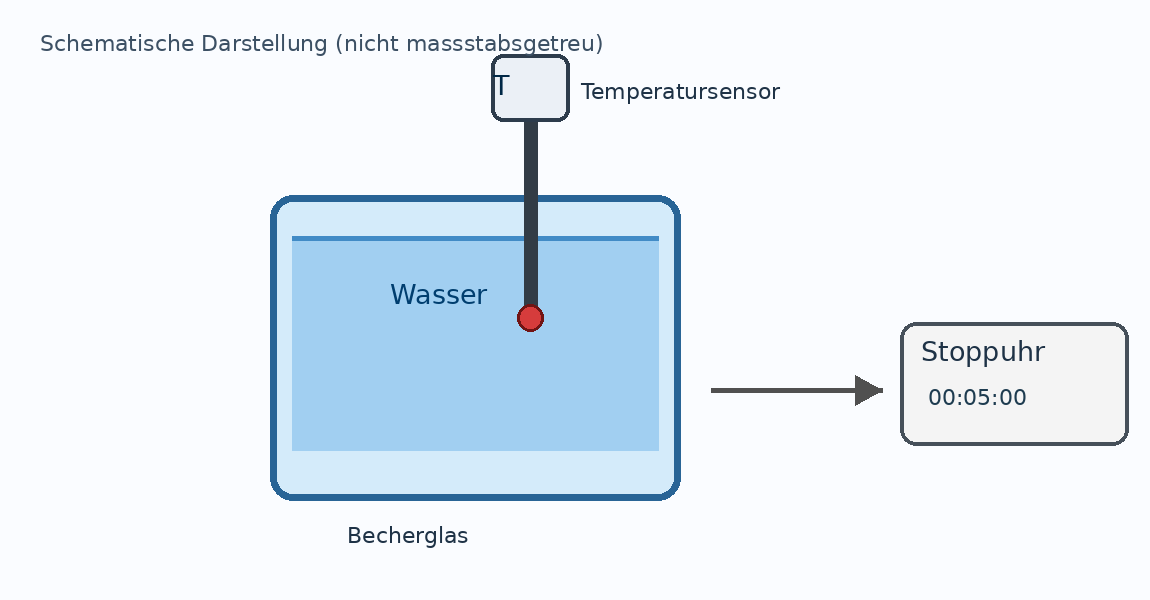
\includegraphics[width=.68\linewidth]{bilder/messaufbau.png}
  \caption{Schematischer Messaufbau (Illustration, keine Fotografie)}
  \label{fig:aufbau}
\end{figure}

\section{Ergebnisse}
Tabelle~\ref{tab:werte} zeigt die beispielhaften Messdaten.
\begin{table}[htbp]
  \centering
  \caption{Beispielhafte Messreihe, keine echten Labordaten}
  \label{tab:werte}
  \begin{tabular}{rr}
    \toprule
    Zeit (min) & Temperatur (\si{\degreeCelsius}) \\
    \midrule
    0  & 65,0 \\
    5  & 58,4 \\
    10 & 52,4 \\
    15 & 47,8 \\
    20 & 44,1 \\
    \bottomrule
  \end{tabular}
\end{table}

Die Abnahme der Temperatur wird berechnet als
\begin{equation}\label{eq:differenz}
  \Delta T = T_{\mathrm{Start}} - T_{\mathrm{Ende}}.
\end{equation}
Mit Gleichung~\eqref{eq:differenz} ergibt sich hier
\(\Delta T = \qty{20.9}{\kelvin}\).

\section{Diskussion}
Die Messreihe ist didaktisch erfunden und daher keine
wissenschaftliche Evidenz. Bei echten Messungen müssen
Messunsicherheiten dokumentiert werden \parencite{jcgm2008}.

\section{Fazit}
Alle grundlegenden Elemente einer kurzen Forschungsarbeit
sind demonstriert. Eine echte Arbeit benoetigt eigene Daten,
eine kritische Auswertung und korrekt belegte Aussagen.

\printbibliography[heading=bibintoc,title={Quellenverzeichnis}]
\appendix
\section{Messprotokoll}\label{anh:protokoll}
\begin{enumerate}
  \item Sensor prüfen.
  \item Stoppuhr starten.
  \item Alle fünf Minuten ablesen.
\end{enumerate}

\end{document}
